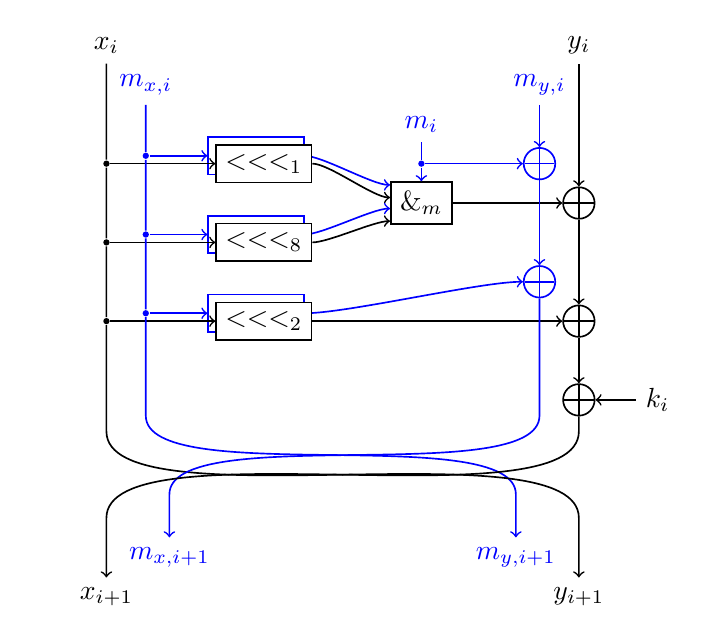
\begin{tikzpicture}
	[line width=0.6,trim left,
	box/.style = {
		draw,
		fill=white
	},
	loosewire/.style = {
		looseness=0.5,
	},
	xor/.style = {
		draw, circle, inner sep=0cm, minimum size=0.4cm,
		append after command = {
			[shorten >=\pgflinewidth, shorten <=\pgflinewidth,]
			(\tikzlastnode.north) edge (\tikzlastnode.south)
			(\tikzlastnode.east) edge (\tikzlastnode.west)
		}
	},
	xorblue/.style = {
		draw=blue, circle, inner sep=0cm, minimum size=0.4cm,
		append after command = {
			[shorten >=\pgflinewidth, shorten <=\pgflinewidth,]
			(\tikzlastnode.north) edge[draw=blue] (\tikzlastnode.south)
			(\tikzlastnode.east) edge[draw=blue] (\tikzlastnode.west)
		}
	},
	circ/.style = {
		draw, circle, inner sep=0cm, minimum size=0.4cm
	},
	dot/.style = {
		fill, circle, inner sep=0cm, minimum size=0.08cm
	}]
	
	%Draw nodes
	\node at (1,7.5) (xin) {$x_i$};
	\node[text=blue] at (1.5,7) (mx) {$m_{x,i}$};
	\node at (7,7.5) (yin) {$y_i$};
	\node[text=blue] at (6.5,7) (my) {$m_{y,i}$};
	\node[text=blue] at (5,6.5) (mi) {$m_i$};
	
	\node[dot,fill=blue] at (1.5,6.1) (d1m) {};
	\node[dot] at (1,6) (d1) {};
	\node[dot,fill=blue] at (1.5,5.1) (d2m) {};
	\node[dot] at (1,5) (d2) {};
	\node[dot,fill=blue] at (1.5,4.1) (d3m) {};
	\node[dot] at (1,4) (d3) {};
	
	\node[dot,fill=blue] at (5,6) (d4m) {};
	
	\node[box, draw=blue] at (2.9,6.1) (S1m) {$<<<_1$};
	\node[box] at (3,6) (S1) {$<<<_1$};
	\node[box, draw=blue] at (2.9,5.1) (S2m) {$<<<_8$};
	\node[box] at (3,5) (S2) {$<<<_8$};
	\node[box, draw=blue] at (2.9,4.1) (S3m) {$<<<_2$};
	\node[box] at (3,4) (S3) {$<<<_2$};
	
	\node[xorblue] at (6.5,6) (x1m) {};
	\node[xor] at (7,5.5) (x1) {};
	\node[xorblue] at (6.5,4.5) (x2m) {};
	\node[xor] at (7,4) (x2) {};
	\node[xor] at (7,3) (x3) {};
	
	\node[box] at (5,5.5) (AND) {$\&_m$};
	\node at (8,3) (k) {$k_i$};
	
	\node at (1, 0.5) (xout) {$x_{i+1}$};
	\node[text=blue] at (1.8, 1) (mxout) {$m_{x,i+1}$};
	
	\node at (7, 0.5) (yout) {$y_{i+1}$};
	\node[text=blue] at (6.2, 1) (myout) {$m_{y,i+1}$};
	
	\coordinate (cright) at (7, 2.6);
	\coordinate (cleft) at (1, 2.6);
	\coordinate (cright2) at (7, 1.5);
	\coordinate (cleft2) at (1, 1.5);
	\coordinate (crightm) at (6.5, 2.8);
	\coordinate (cleftm) at (1.5, 2.8);
	\coordinate (crightm2) at (6.2, 1.8);
	\coordinate (cleftm2) at (1.8, 1.8);
	
	%Draw wires
	\draw[->,draw=blue] (d1m) -- (S1m);
	\draw[->] (d1) -- (S1);
	
	\draw[loosewire,->,draw=blue] (S1m.east) to[out=0, in=180] (AND.150);
	\draw[loosewire,->] (S1.east) to[out=0, in=180] (AND.170);
	\draw[->,draw=blue] (d2m) -- (S2m);
	\draw[->] (d2) -- (S2);
	
	\draw[loosewire,->,draw=blue] (S2m.east) to[out=0, in=180] (AND.190);
	\draw[loosewire,->] (S2.east) to[out=0, in=180] (AND.210);
	
	\draw[->] (AND) -- (x1);
	
	\draw[->,draw=blue] (d3m) -- (S3m);
	\draw[->] (d3) -- (S3);
	
	\draw[loosewire,->,draw=blue] (S3m.east) to[out=0,in=180] (x2m);
	\draw[->] (S3.east) -- (x2);
	
	\draw[loosewire,->,draw=blue] (mx) -- (d1m) -- (d2m) -- (d3m)
	-- (cleftm) to[out=270, in=90] (crightm2) -- (myout.north);
	\draw[loosewire,->] (xin) -- (d1) -- (d2) -- (d3)
	-- (cleft) to[out=270, in=90] (cright2) -- (yout.north);
	
	
	\draw[->,draw=blue] (my) -- (x1m);
	\draw[->] (yin) -- (x1);
	\draw[->,draw=blue] (x1m) -- (x2m);
	\draw[->] (x1) -- (x2);
	\draw[->] (x2) -- (x3);
	
	\draw[loosewire,->,draw=blue] (x2m) -- (crightm) to[out=270, in=90] (cleftm2) -- (mxout.north);
	\draw[loosewire,->] (x3) -- (cright) to[out=270, in=90] (cleft2) -- (xout.north);
	\draw[->] (k.west) -- (x3);
	
	%additional wires for mask
	\draw[->,draw=blue] (mi) -- (d4m) -- (AND);
	\draw[->,draw=blue] (d4m) -- (x1m.west);
	
	%draw black boxes again to show them in front of blue arrows
	\node[box] at (3,6) (S1) {$<<<_1$};
	\node[box] at (3,5) (S2) {$<<<_8$};
	\node[box] at (3,4) (S3) {$<<<_2$};
	
\end{tikzpicture} 

